Uno de los principales factores limitantes del modelo a escala del vehículo WIG construido es el hecho de que no cuenta con una planta propulsora. Esto implica que, para poder determinar sus características de vuelo será necesario diseñar unas pruebas que permitan la propulsión del vehículo mediante fuerzas externas al mismo. Para ello, será necesario ingeniar un sistema que permita dotar al modelo de una velocidad inicial conocida, evitando en la medida de lo posible que este sistema externo afecte notablemente a la eficiencia y a los resultados de las pruebas.

En las siguientes subsecciones se expondrá cuál es el sistema ideado para propulsar el modelo, indicando también las pequeñas modificaciones que se han debido realizar sobre el mismo. A continuación, se explicará cómo y dónde se han llevado a cabo las pruebas y se proporcionarán los resultados obtenidos, que serán sometidos a un discusión crítica y justificada.


\subsection{Preparación}
\label{sec:tests:preparation}

\subsubsection{Concepción de las pruebas}
\label{sec:tests:preparation:conception}

Las principales dificultades que surgen a la hora de determinar las prestaciones del modelo son consecuencia de la decisión de haber construido un modelo no autopropulsado, por motivos comentados anteriormente. Si hubiese incorporado una pequeña planta propulsora, habría sido suficiente con establecer una potencia y medir una serie de prestaciones como la velocidad o la separación vertical, entre otras.

Sin embargo, esta carencia obliga a ser más creativos e idear una serie de pruebas alternativas. En lugar de asociar una serie de potencias generadas por la planta propulsora a las correspondientes velocidades alcanzadas por el modelo, se proponen otro tipo de pruebas en las que se asociará un impulso inicial conocido a la distancia recorrida por el modelo hasta su detención.

Asimismo, durante las pruebas se prestará especial atención a un factor difícilmente cuantificable pero fácilmente observable: la estabilidad del modelo para distintas velocidades (es decir, para distintos impulsos iniciales). Por ello, las pruebas se grabarán en vídeo para un posterior análisis detallado de la trayectoria del vehículo, así como de las posibles variaciones de altitud y del ángulo de cabeceo durante el vuelo.


\subsubsection{Mecanismo de lanzamiento}
\label{sec:tests:preparation:mechanism}

Al no contar con planta propulsora, el modelo se debe poner en movimiento mediante la acción de alguna fuerza externa. El método más natural y sencillo es lanzarlo manualmente, pero esto imposibilita la cuantificación de las prestaciones del modelo, ya que resulta muy difícil lanzarlo con la velocidad y el ángulo deseados.

Así pues, se ha optado por el uso de un resorte para dotar al modelo de una velocidad inicial. El resorte acumulará una energía potencial elástica (calculable) que se transformará en energía cinética, haciendo salir al modelo de su posición de reposo. Además, si el mecanismo de lanzamiento se diseña cuidadosamente, es posible lanzar el vehículo con el ángulo deseado e incluso dotarlo de una velocidad inicial deseada que pueda resultar de especial interés.

Aunque se haya hablado del uso de un resorte, esto no implica necesariamente el uso de un muelle metálico. La definición técnica y más amplia de resorte es la siguiente \cite{ref:resorte}: \emph{operador elástico capaz de almacenar energía y desprenderse de ella sin sufrir deformación permanente cuando cesan las fuerzas o la tensión a las que es sometido}. Dentro de esta definición entra también el concepto de cinta elástica, que es lo que se utilizará para efectuar el lanzamiento del modelo (\rfig{cintaelastica}).

Uno de los extremos de la cinta se fijará al suelo (o a la superficie sobre la que se vaya a lanzar el modelo), mediante cinta adhesiva, tal y como se muestra en la \rfig{cintapreparada}. En el otro extremo se realiza un agujero que permitirá “anclar” el modelo a la cinta (será necesario realizar adaptaciones en el modelo, como se detallará en la siguiente subsección). La cinta se someterá a tensión manualmente, incrementando su longitud, de modo que almacenará energía potencial elástica. Realmente, no se estirará de la cinta, sino del modelo, que estará unido a ésta. Al liberarlo, la cinta recuperará su longitud original, transmitiendo la energía potencial elástica que había acumulado al modelo, que se liberará de la cinta e iniciará el vuelo con una velocidad determinada, en función de cuánto se haya estirado la cinta elástica. Este incremento de longitud se medirá hasta el punto correspondiente al orificio realizado en el extremo de la cinta.


\subsubsection{Adaptación del modelo}
\label{sec:tests:preparation:adaptation}

Como ya se ha anticipado, es necesario incorporar al modelo un elemento que le permita permanecer unido a la cinta elástica mientras ésta está en tensión y que, al mismo tiempo, permita que el vehículo se libere de la cinta una vez toda su energía potencial elástica haya sido liberada.

Para ello, se ha incorporado un gancho o alcayata en la parte inferior delantera del fuselaje del modelo, que sobresale ligeramente, tal y como se aprecia en la \rmfig{alcayataangulo}{jpg}{110}{ht}{Alcayata en la parte delantera del fuselaje}. Nótese que se le ha dotado de un cierto ángulo de ataque con el objetivo de que se pueda liberar de la cinta elástica con una pérdida mínima de energía.

Aunque la alcayata utilizada cuenta con un roscado en la parte que ha sido introducida en el fuselaje, esto no es suficiente para mantenerla unida al modelo adecuadamente, debido a las características del poliestireno expandido. Por ello, tal y como se observa en la \rfig{alcayataarandela}, se ha hecho uso de cola de contacto (la misma que la utilizada para unir las partes del modelo) y además se ha incorporado una arandela de plástico, con el objetivo de evitar que la alcayata rompa el material del modelo cuando éste se encuentra unido a la cinta elástica en tensión. Al distribuir cola alrededor de la alcayata y de la arandela, la tensión ejercida por la alcayata sobre el modelo se distribuye y se evitan posibles daños.

Tras esta incorporación, la masa del modelo asciende hasta los 34 gramos y su centro de gravedad se adelanta hasta situarse a 27 cm del extremo frontal del fuselaje.


\subsubsection{Calibración de la cinta elástica}
\label{sec:tests:preparation:calibration}

Aunque la cinta elástica no es un muelle propiamente dicho, su comportamiento sí es equivalente al de un resorte y por lo tanto cabe esperar que se ajuste a la ley de Hooke:
\eq{hooke}{
F = -k\delta
}

Es interesante estimar el valor de la constante elástica $k$, ya que permitirá conocer de inmediato la fuerza ejercida sobre el modelo si se conoce la longitud $\delta$ que se ha elongado la cinta elástica. Además, conocer esta constante también puede servir para calcular la energía potencial elástica que se transfiere al modelo en forma de energía cinética y por lo tanto su velocidad inicial.

Sin embargo, esta información también se puede obtener a partir de las mismas pruebas, que van a ser grabadas en vídeo. Es por ello que el objetivo principal de la calibración de la cinta elástica no es tanto determinar el valor exacto de su contante, sino comprobar que efectivamente se comporta como un resorte y que su respuesta es lineal, es decir, que para una elongación de por ejemplo 50 cm, la fuerza ejercida sobre el modelo sea el doble que la ejercida para una elongación de 25 cm.

Para comprobar esta hipótesis, se ha colocado la cinta elástica en posición vertical y se le han colgado una serie de pesos, que se han ido variando hasta que la cinta se ha elongado hasta la distancia deseada en cada caso. Los resultados obtenidos se proporcionan en la Tabla \ref{tab:cintaelastica}.

\begin{table}[ht]
\centering
\caption{Experimentos realizados para la calibración de la cinta elástica.}
\label{tab:cintaelastica}
\begin{tabular}{llll}
\toprule
\# Experimento & Masa [kg]       & Peso [N]       & $\delta$ [cm] \\ \midrule
1              & $1.222$         & $11.99$        & 30          \\
2              & $1.511$         & $14.82$        & 40          \\
3              & $1.710$         & $16.78$        & 45          \\
4              & $1.886$         & $18.50$        & 50         \\ \bottomrule
\end{tabular}
\end{table}

A partir de esta información, se ha obtenido la recta que mejor se ajusta a los datos (\rfig{ajustek}) y se ha observado que el comportamiento de la cinta elástica es altamente lineal, comportándose como un resorte de constante elástica $0.37$ N/cm.

\mfig{ajustek}{pdf}{90}{ht}{Obtención de la constante elástica mediate ajuste de los datos obtenidos por una recta}

\subsection{Desarrollo y resultados}
\label{sec:tests:results}

La primera de las pruebas ha consistido en lanzar el vehículo para determinar su respuesta en estabilidad a varias velocidades. Para ello, se han realizado varios lanzamientos, tensionando la cinta elástica hasta alcanzar elongaciones de 30, 40 y 50 cm respectivamente. En la \rmfig{lanzamientoperfil}{jpg}{110}{ht!}{Fotogramas correspondientes a la fase inicial de lanzamiento del modelo} se muestran cuatro fotogramas consecutivos correspondientes a uno de los lanzamientos realizados en esta primera fase de las pruebas. Entre el primero y el último fotograma han transcurrido $0.12$ segundos.

Las pruebas se han realizado al aire libre en una zona espaciosa y sobre una superficie aparentemente lisa. A pesar de que no soplaba el viento, o si soplaba lo hacía con una fuerza imperceptible, se han tomado medidas lanzando el modelo en diferentes direcciones con el objetivo de corroborar que el viento no influya en los resultados.

Todas las pruebas de interés han sido grabadas con una cámara de vídeo a 25 fps (fotogramas por segundo). A partir de estos vídeos, se podrán medir algunos parámetros como la velocidad inicial del modelo determinando la distancia recorrida entre varios fotogramas consecutivos o la separación vertical entre el suelo y el modelo durante el vuelo.

De la primera fase de pruebas se puede estimar el comportamiento del modelo bajo la influencia del efecto suelo. Para determinar si el efecto suelo supone realmente una ventaja considerable, se ha realizado una segunda tanda de pruebas en las que el modelo no se lanza a ras de suelo, sino des de una cierta altura. El objetivo de estas pruebas es determinar cuánto tarda el modelo en alcanzar de nuevo la altura desde la que ha sido lanzado y la distancia recorrida durante ese intervalo de tiempo, y compararla con los resultados correspondientes a las pruebas realizadas bajo la influencia del efecto suelo.

En este caso, las pruebas se han realizado en otra zona resguardada del viento pero de dimensiones menores (\rmfig{lanzamientonoge}{jpg}{120}{bt}{Configuración experimental para el estudio del comportamiento del modelo fuera de la zona de influencia del efecto suelo}), por lo que por razones de espacio tan solo se han realizado lanzamientos para una elongación de la cinta elástica de 30 cm. En cualquier caso, haber lanzado el modelo con la cinta más tensionada habría resultado peligroso debido a la velocidad vertical que puede llegar a alcanzar en cuanto llega al suelo. Por este mismo motivo, la altura desde la que se ha lanzado es bastante reducida: 20 cm, ya que el modelo ha sufrido algunos daños en intentos de lanzarlo desde alturas superiores. Sin embargo, se considera que 20 cm son suficientes para que la aeronave opere fuera de la zona de influencia del efecto suelo, ya que la separación vertical estimada es inferior a 5 cm, como se verá en el apartado de resultados de la siguiente subsección.

Por último, además de estudiar el comportamiento del vehículo operando dentro y fuera de la zona de influencia del efecto suelo, se ha querido también estudiar cómo se ve modificada su respuesta en estabilidad a variaciones de peso y del centro de gravedad. Para ello, se ha recurrido al uso de monedas, que situadas sobre el fuselaje del modelo permiten modificar su peso y desplazar el centro de gravedad en la dirección deseada. Se han probado varios casos, entre ellos la incorporación de un peso de 25 gramos (incrementando el peso total del modelo hasta los 59 gramos) sobre el centro de gravedad, y la incorporación de este mismo peso delante del centro de gravedad, haciendo que éste se desplace hacia delante.

\FloatBarrier

\subsubsection{Alcance con efecto suelo}
\label{sec:tests:results:ge}

La primera tanda de pruebas ha consistido en lanzar el modelo estirando la cinta elástica una cierta distancia. En este caso, el modelo se lanza a ras de suelo, por lo que cabe esperar que vuele dentro de la zona de influencia del efecto suelo. El dato de mayor interés es la distancia recorrida por el vehículo en cada caso. En la Tabla \ref{tab:test1geN} se proporciona dicha información para cada una de las pruebas realizadas.

\begin{table}[ht]
  \centering
  \caption{Distancia recorrida por el modelo (en metros) bajo la influencia del efecto suelo. Lanzamientos realizados en sentido \textbf{norte}.}
  \label{tab:test1geN}
  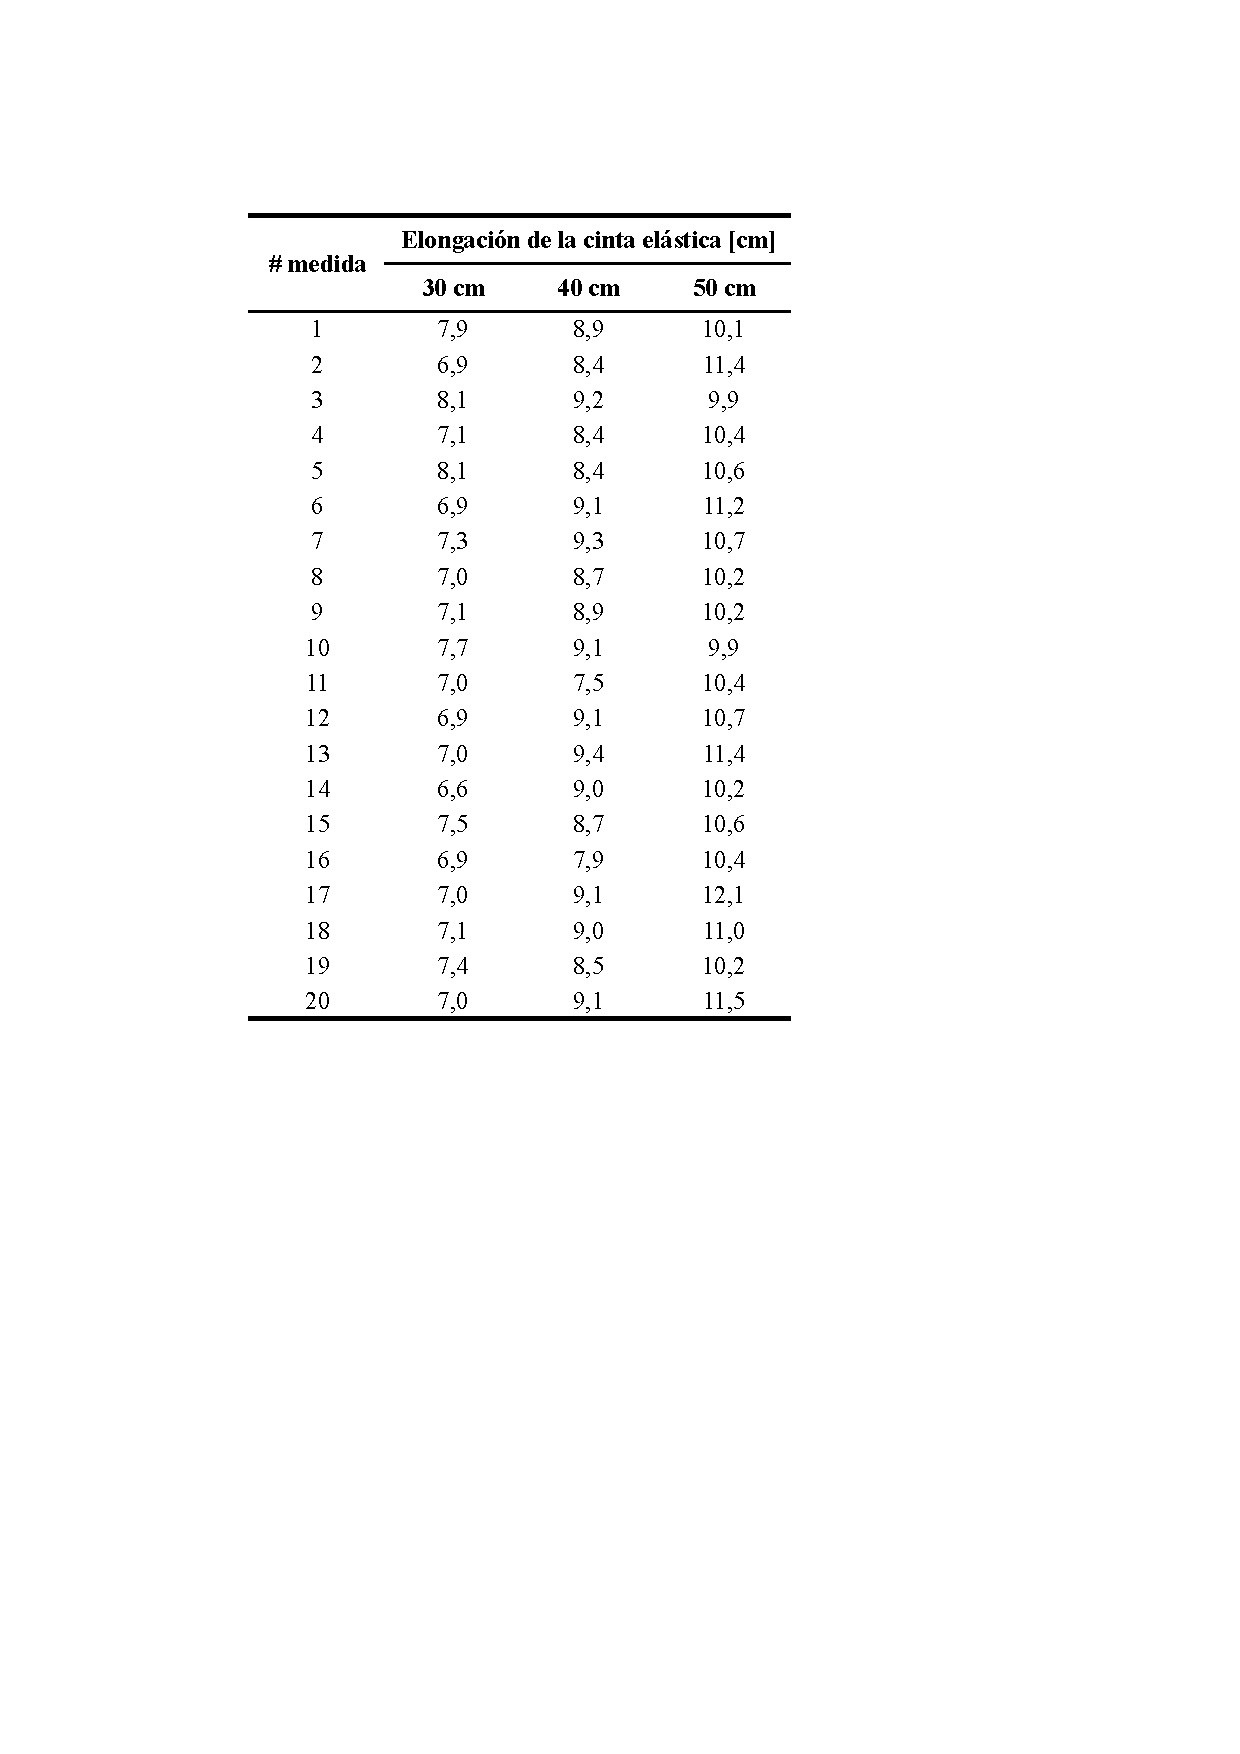
\includegraphics[width=0.5\linewidth]{masmedidasN.pdf}
\end{table}

Se ha repetido cada prueba veinte veces, con el objetivo de eliminar posibles errores aleatorios que desvirtúen el resultado final. Sin embargo, como las pruebas no se realizan en un recinto cerrado, es posible que todos los resultados se hayan visto afectados por un error sistemático inducido por el viento que, aunque inapreciable para el ser humano, puede afectar considerablemente a un objeto tan ligero. Por ello, se han repetido las pruebas anteriores pero lanzando el modelo en sentido opuesto. Tanto en el caso anterior como en éste el modelo ha volado en línea recta, por lo que se considera que la dirección elegida (Norte-Sur) es la misma dirección en la que soplaba el viento durante la realización de las pruebas. Los resultados obtenidos en este caso se detallan en la Tabla \ref{tab:test1geS}.

\begin{table}[ht]
  \centering
  \caption{Distancia recorrida por el modelo (en metros) bajo la influencia del efecto suelo. Lanzamientos realizados en sentido \textbf{sur}.}
  \label{tab:test1geS}
  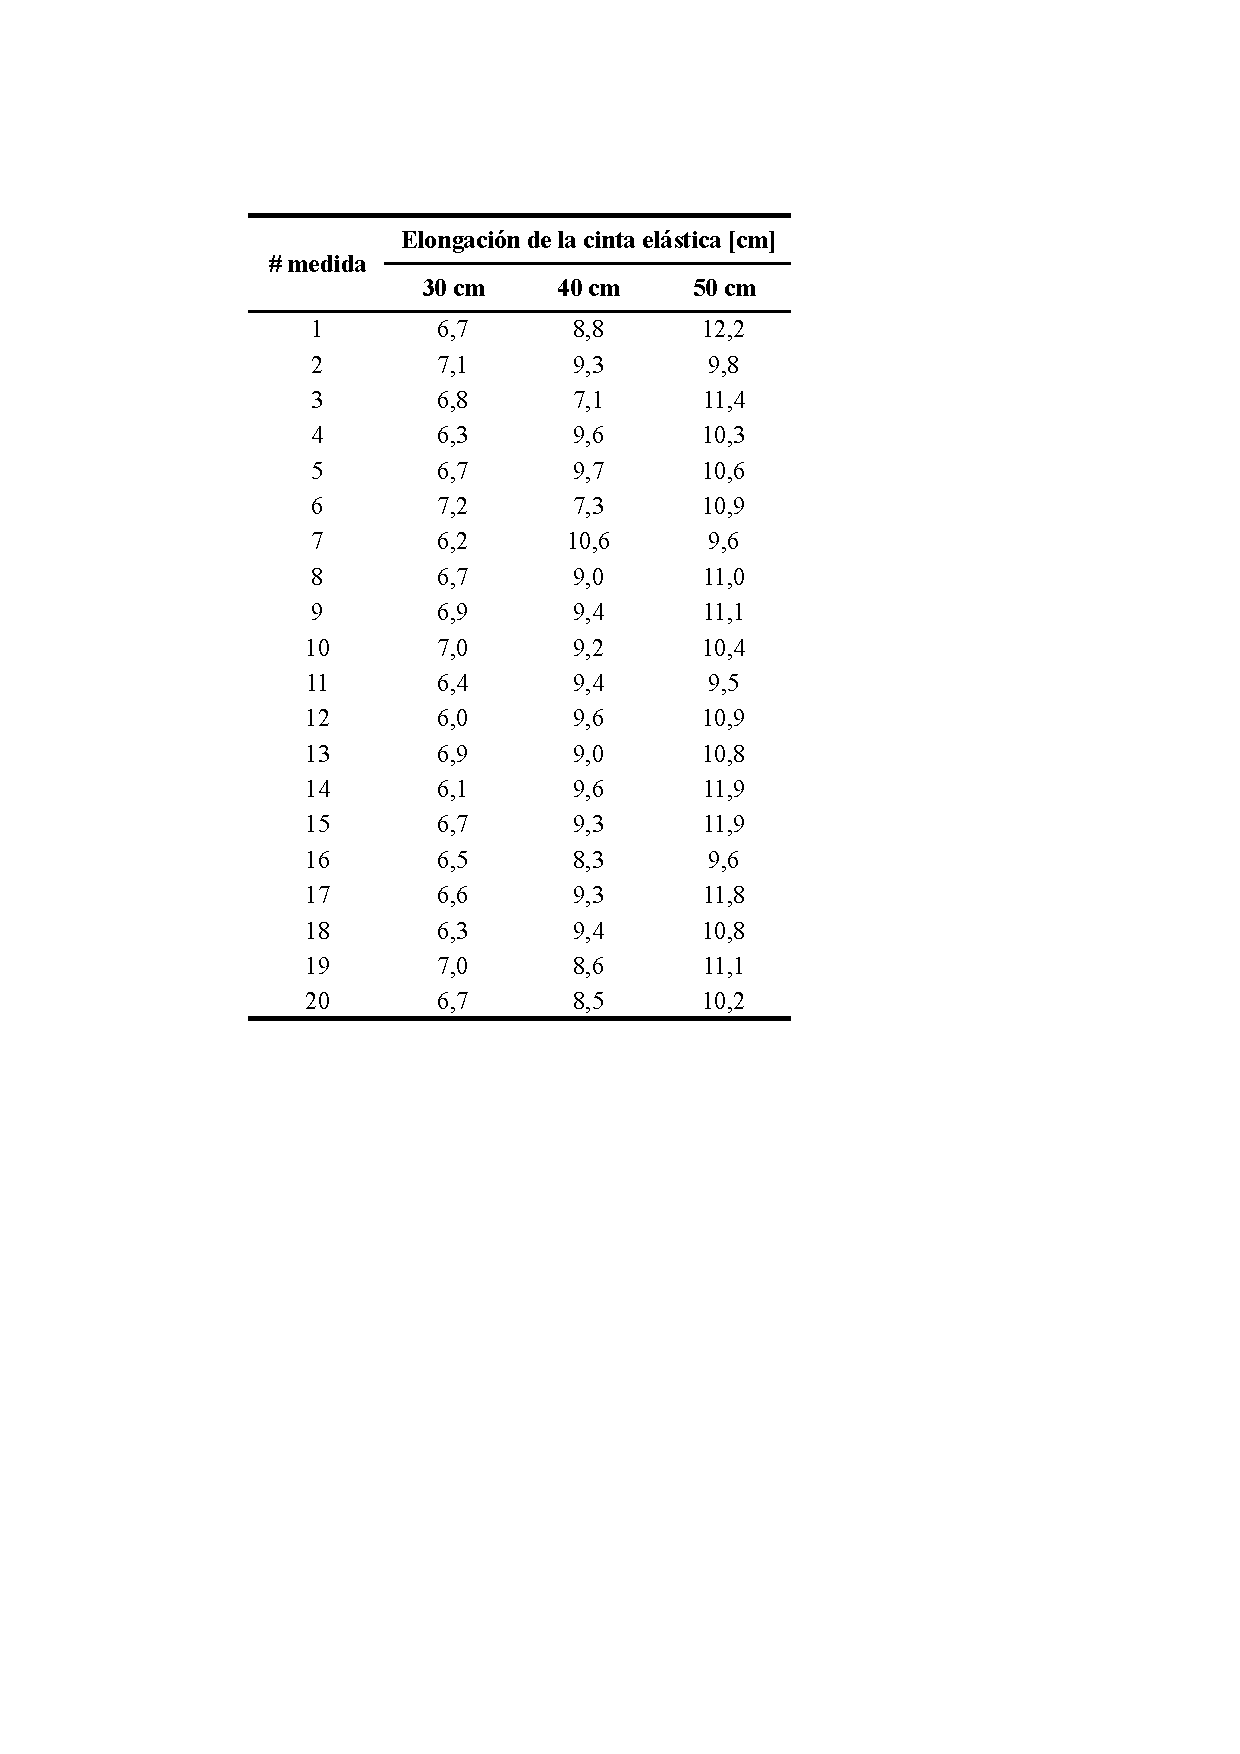
\includegraphics[width=0.5\linewidth]{masmedidasS.pdf}
\end{table}

De los resultados registrados se puede determinar si existe o no un error significativo sistemático ocasionado por el efecto del viento. Para facilitar esta tarea, se han representado los datos de las tablas \ref{tab:test1geN} y \ref{tab:test1geS} en la \rmfig{medidas}{pdf}{80}{h}{Visualización gráfica de las distintas medidas realizadas para una elongación de la cinta elástica de a) 30 cm, b) 40 cm y c) 50 cm}.

De dichas gráficas se puede intuir que no existen diferencias abismales entre los resultados obtenidos al lanzar el modelo en una dirección u otra. Sin embargo, esta visualización no nos permite aseverar si las diferencias que puedan existir entre una serie de datos y la correspondiente a lanzamientos en sentido opuesto es lo suficientemente pequeña para poder considerarla despreciable. Por ello, se procede obtener el valor medio de cada una de las configuraciones de lanzamiento.

En primer lugar, es conveniente identificar posibles valores atípicos que pertenezcan a una población diferente del resto de la muestra establecida, como por ejemplo lanzamientos en los que el viento sí tuvo una influencia significativa o lanzamientos en los que un incorrecto ángulo de ataque inicial alteró las prestaciones de estabilidad del modelo.

Para identificar y descartar estos datos, el primer paso consiste en hallar el primer y tercer cuartil de cada una de las series, definiéndose éstos como sendas medianas de la primera y segunda mitad de los datos ordenados en sentido creciente. Por ejemplo, para hallar los cuartiles del caso correspondiente a los lanzamientos realizados en sentido norte con una elongación de la cinta elástica de 30 cm, como existen 20 datos, se dividen en dos mitades de 10 datos cada una, y la mediana de cada una de estas mitades se obtiene como la media del quinto y el sexto dato. En este ejemplo, se obtienen un primer y tercer cuartil de $6.98$ y $7.33$ metros respectivamente.

Una vez hallados los cuartiles, se procede a determinar el rango intercuartil como la diferencia entre el tercer y el primer cuartil. En el ejemplo anterior se tiene:
\eq{iqr}{
IQR = Q_3 - Q_1 = 7.33 - 6.98 = 0.35
}

Una vez hallado el rango intercuartil, se pueden definir sendos límites inferior y superior por debajo o por encima de los cuales los valores existentes se considerarán atípicos. Habitualmente, cuando se busca identificar valores atípicos leves, dichos límites se calculan de la siguiente manera:
\eq{liminf}{
$límite inferior $= Q_1 - 1.5IQR; \qquad $límite superior $= Q_3 + 1.5IQR
}

En el caso de una elongación de la cinta elástica de 30 cm, se obtienen unos límites de $6.45$ y $7.85$ metros. De este modo, se pueden descartar un total de tres de los veinte valores tomados por ser considerados atípicos leves. Concretamente, se han descartado las mediciones primera ($7.9$ m), tercera ($8.1$ m) y quinta ($8.1$ m).

Procediendo de forma análoga para las cinco series de medidas restantes, se obtienen los resultados sintetizados en la Tabla \ref{tab:stats}.

\begin{table}[ht]
  \centering
  \caption{Valores estadísticos de interés acerca de las distintas series de datos obtenidas.}
  \label{tab:stats}
  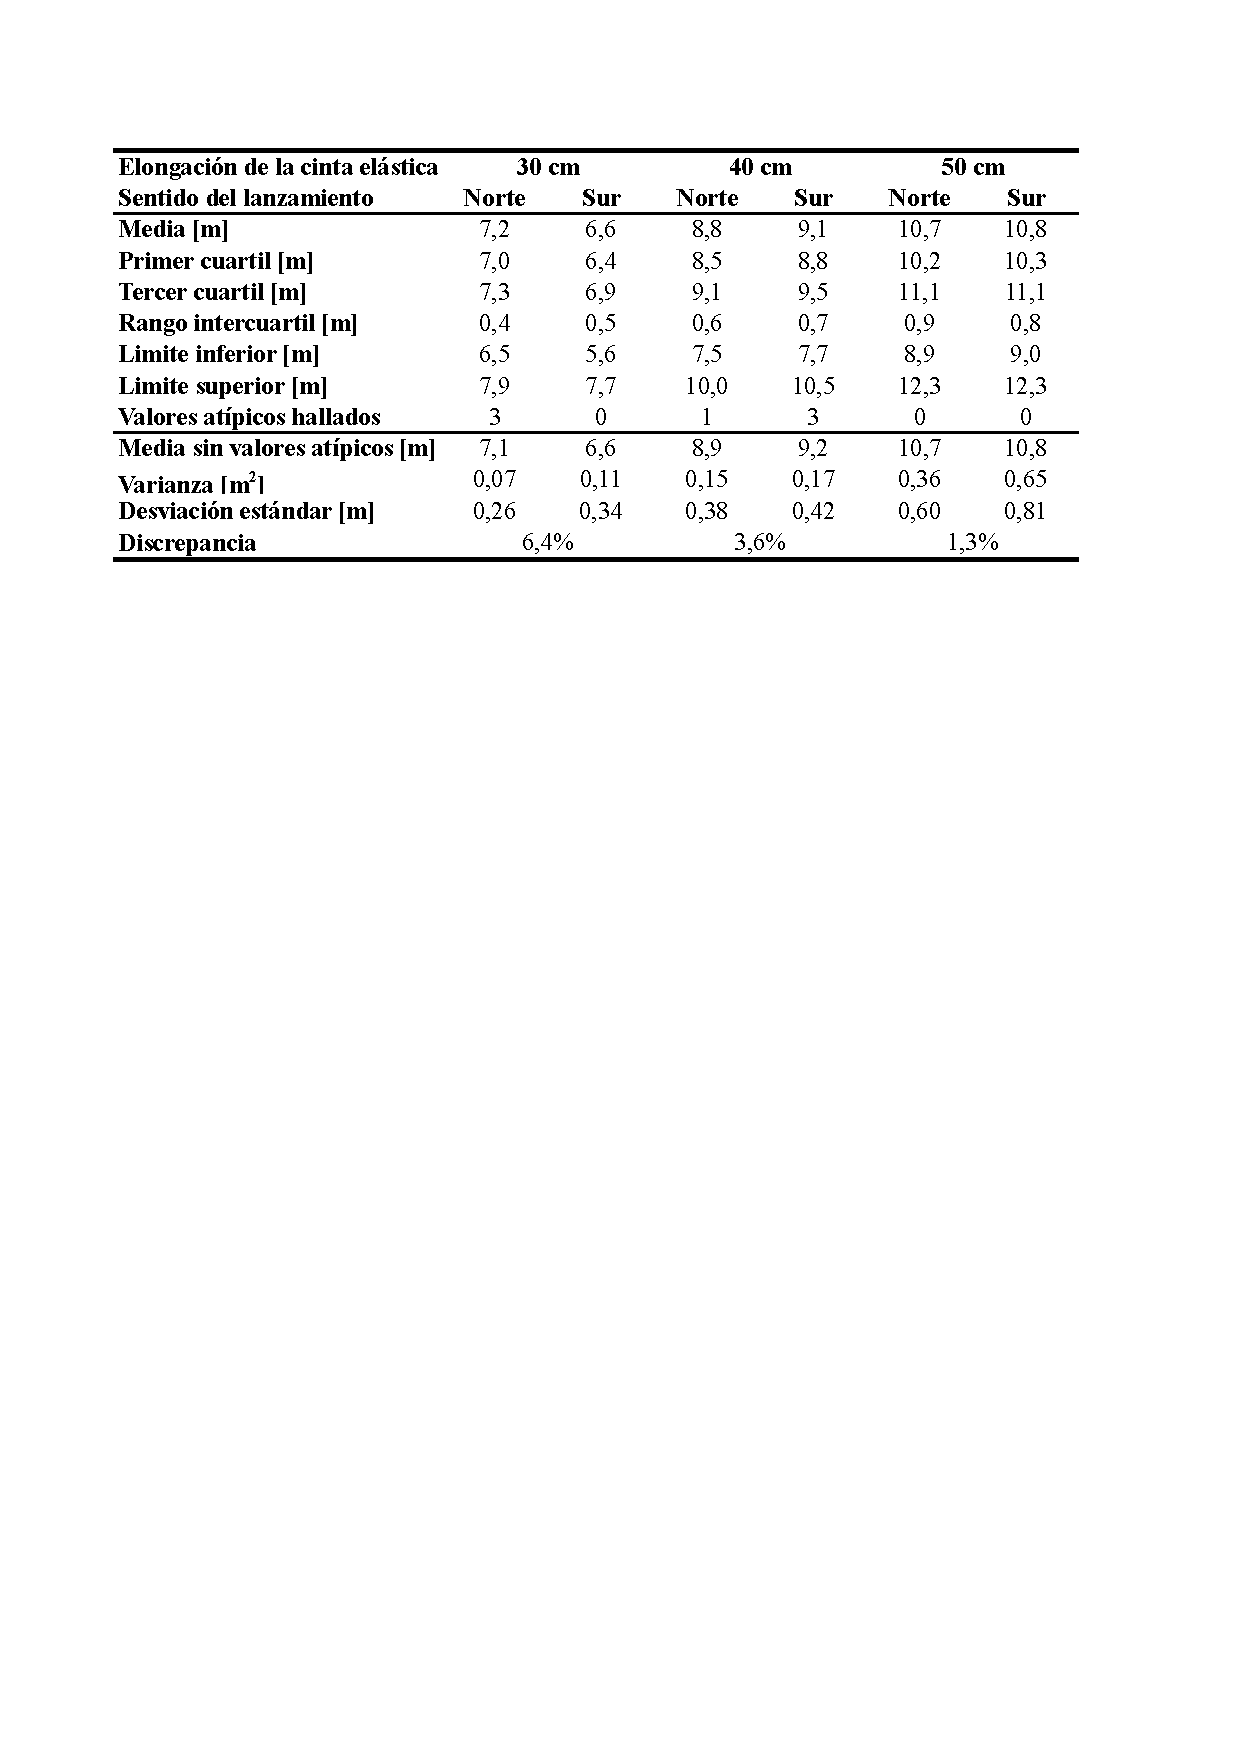
\includegraphics[width=0.95\linewidth]{stats.pdf}
\end{table}

En la tabla también se han incluido la media, la varianza y la desviación estándar de las distintas series una vez eliminados los valores atípicos, así como la discrepancia existente entre los lanzamientos en sentido sur y sentido norte, calculada como la diferencia entre la media de un sentido y el opuesto dividida entre la media de ambos valores. Por ejemplo, en el caso de una elongación de la cinta elástica de 30 cm se ha procedido de la siguiente manera:

\eq{discrepancia}{
$discrepancia $= \frac{7.1 - 6.6}{\frac{7.1+6.6}{2}} = 0.064 = 6.4\%
}

Se considera que valores de discrepancia inferiores al 5\% permiten aseverar que no existen diferencias estadísticamente significativas entre los lanzamientos en sentido norte y en sentido sur. Como se puede observar, las discrepancias en los casos correspondientes a elongaciones de la cinta elástica de 40 y 50 cm son inferiores al 5\%, pero no ocurre así para una elongación de 30 cm. Es interesante observar cómo a medida que el modelo es lanzado con mayor fuerza y por lo tanto mayor velocidad inicial, la discrepancia y, por tanto, el efecto del viento, va disminuyendo, seguramente debido a que el peso relativo del viento es menor a medida que aumenta la velocidad del modelo.

Como ya se ha comentado en varias ocasiones, el objetivo de este Trabajo de Fin de Grado no es determinar con exactitud las prestaciones de un ekranoplano, lo cual sería imposible de llevar a cabo a estas alturas, después de todas las simplificaciones en el diseño y construcción del modelo, sino más bien determinar si el modelo operando en la zona de influencia del efecto suelo es más competitivo que cuando lo hace fuera de ella. Por ello, se ha decidido relajar el límite máximo de discrepancia permitida, subiéndolo hasta el 10\%, lo cual permitirá disponer de un total de cuarenta medidas válidas para cada una de las tres configuraciones de la cinta elástica: 30, 40 y 50 cm de elongación.

Así pues, se pueden tratar las 40 medidas en su conjunto sin separarlas entre las que han sido realizadas en sentido norte y en sentido sur, obteniendo los valores estadísticos proporcionados en la Tabla \ref{tab:statsall}.

\begin{table}[ht]
  \centering
  \caption{Valores estadísticos de interés para las distintas elongaciones de la cinta elástica.}
  \label{tab:statsall}
  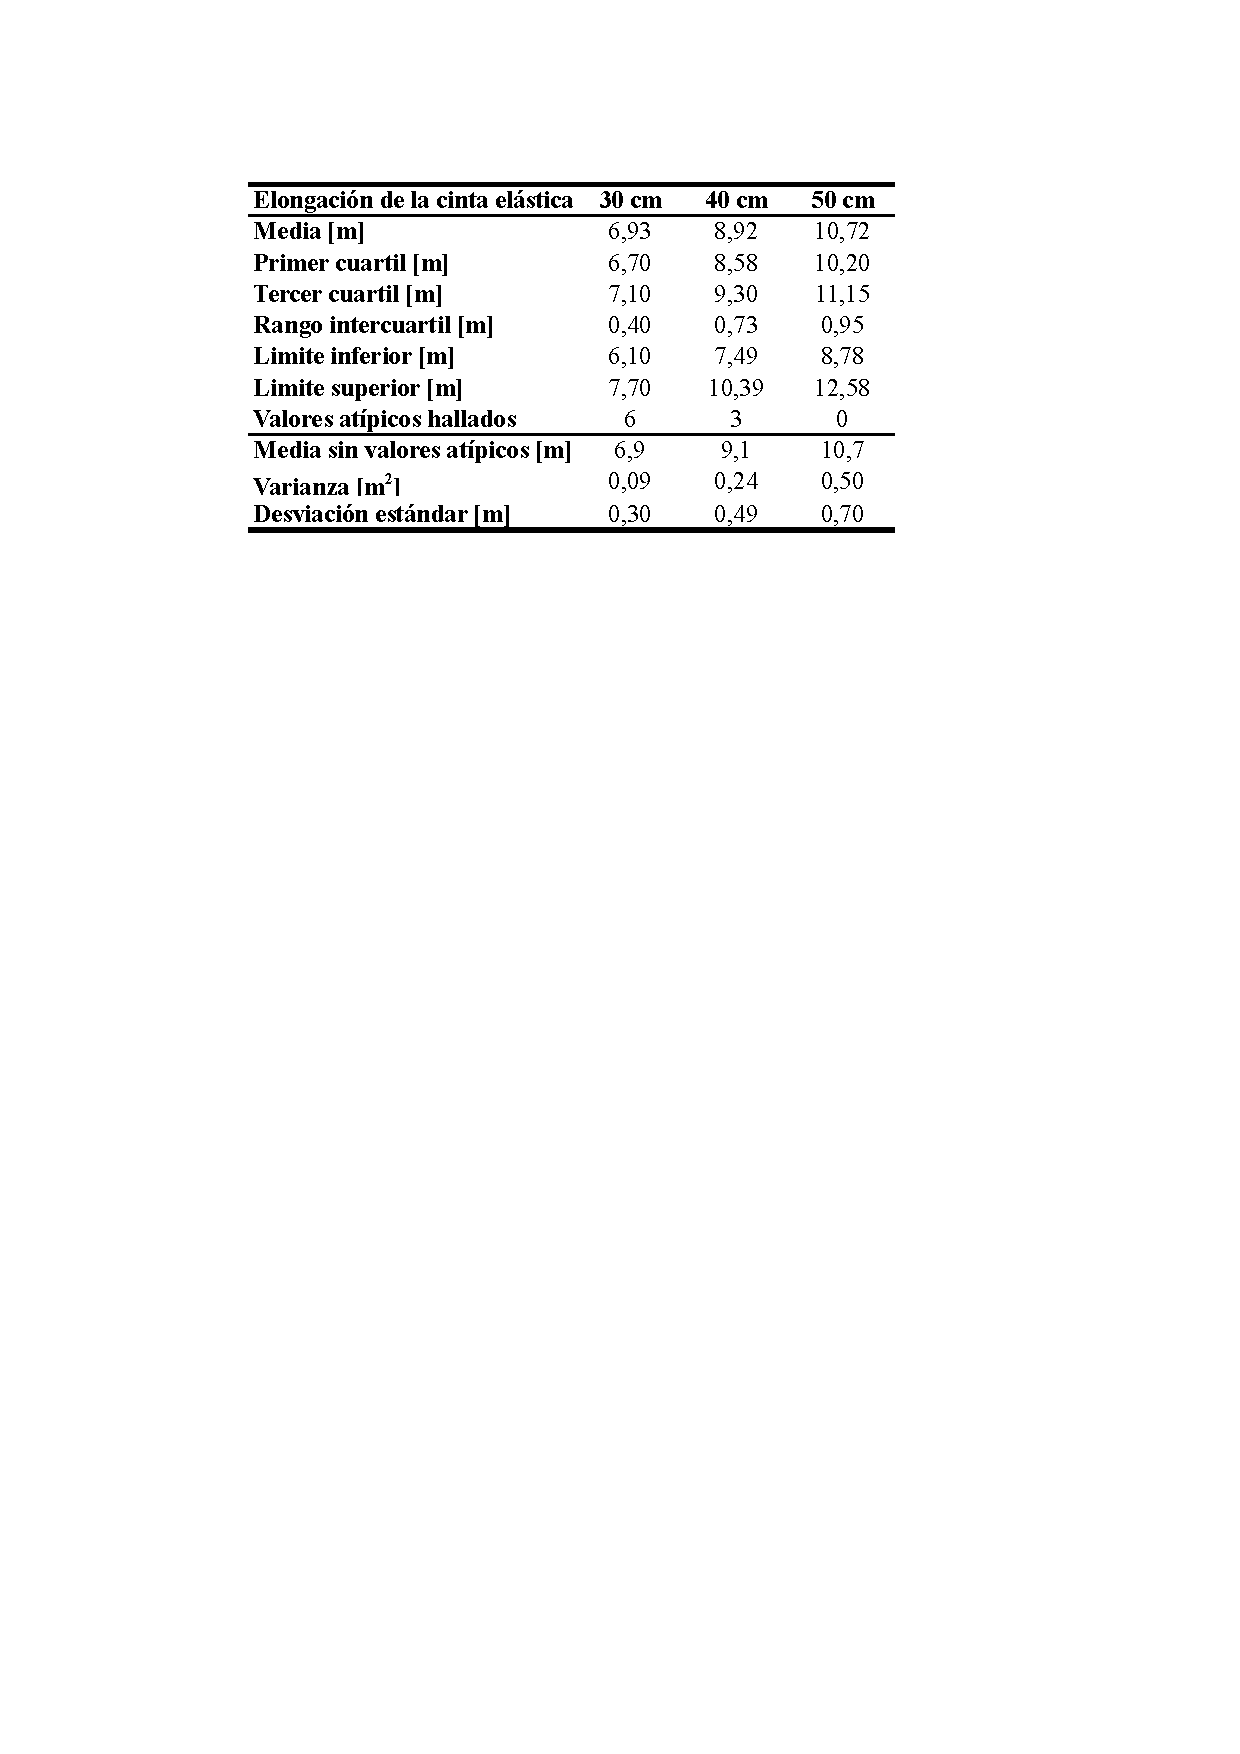
\includegraphics[width=0.65\linewidth]{statsall.pdf}
\end{table}

De ahora en adelante, se podrán utilizar las tres medias obtenidas tras eliminar los valores atípicos para realizar más cálculos y extraer más conclusiones. Así pues, se considera que, cuando la cinta elástica se elonga hasta los 30, 40 y 50 cm, la distancia recorrida por el modelo es, respectivamente, de $6.9$, $9.1$ y $10.7$ metros.

A partir de dicha información se puede determinar la relación existente entre la elongación de la cinta elástica y la distancia recorrida por el modelo. En la \rmfig{test1}{pdf}{100}{ht}{Ajuste mediante una recta de los datos experimentales relativos al lanzamiento del modelo en la zona de influencia del efecto suelo} se observa que se trata de una relación lineal. La ecuación de la recta que mejor se ajusta a los datos experimentales es:
\eq{test1ajuste}{
d = 18.75\delta + 1.38
}
con la distancia recorrida $d$ y la elongación de la cinta elástica $\delta$ ambos en las mismas unidades.

A partir del valor de la constante elástica de la cinta obtenido en la sección \ref{sec:tests:preparation:calibration} es posible estimar la velocidad inicial con la que es lanzado el modelo en cada caso. Para ello, se supone que existe una transformación sin pérdidas de toda la energía potencial elástica de la cinta a energía cinética. Igualando ambas expresiones se tiene:
\eq{epec}{
\frac12 k \delta^2 = U_e = E_C = \frac12 m v^2
}
de donde es posible despejar la velocidad:
\eq{vteorica}{
v = \sqrt{\frac{k}{m}}\delta
}

Recordando que $k=37$ N/m y $m=34$ g, se obtienen velocidades de $9.9$, $13.2$ y $16.5$ m/s para elongaciones de 30, 40 y 50 cm, respectivamente.

Éstas son las velocidades iniciales con las que cabe esperar que haya sido lanzado el modelo en el momento de su separación de la cinta elástica (cuando ésta ya ha perdido toda su energía potencial). Sin embargo, se ha asumido que la transformación de energía es ideal, sin pérdidas, y además se han despreciado las variaciones que hayan podido dar en la energía potencial gravitatoria, ya que el modelo gana cierta altura al ser lanzado a ras de suelo, si bien esta altura es pequeña y el modelo poco pesado por lo que este efecto no debería tener demasiada influencia en los valores de velocidad calculados.

Como no se puede saber a ciencia cierta que las pérdidas de energía producidas durante la separación del modelo respecto de la cinta elástica sean despreciables a la hora de determinar la velocidad mediante este método, se ha procedido a hacer uso de las grabaciones de vídeo del modelo para estudiar visualmente qué distancia recorre el modelo al inicio del lanzamiento en un cierto número de fotogramas (es decir, en un cierto tiempo). De este modo, es posible obtener una estimación más directa de la velocidad inicial y, en caso de que las pérdidas de energía sean relevantes, un valor también más preciso que el calculado teóricamente.

Para estimar la velocidad del modelo a partir de los fotogramas extraídos de las grabaciones de vídeo es imprescindible saber que la cámara graba a 25 fps, o lo que es lo mismo, dos fotogramas consecutivos están espaciados temporalmente entre sí por $40$ ms. La grabación se realiza desde arriba, con la cámara apuntando hacia el suelo, sobre el cual se ha marcado una escala necesaria para poder determinar el espacio recorrido entre fotogramas (\rfig{grabacionarriba}). Los valores de velocidad inicial obtenidos por este método son: $5.0$, $6.3$ y $7.8$ m/s para elongaciones de 30, 40 y 50 cm, respectivamente.

\mfig{grabacionarriba}{jpg}{120}{ht}{Modelo a punto de ser lanzado sobre una superficie en la que se ha marcado una escala}

Evidentemente, el método teórico no es válido en este caso, ya que las pérdidas de energía son tan grandes que la velocidad con la que realmente se lanza el modelo en inferior a la mitad del valor estimado analíticamente. Como ya se ha anticipado, la posible causa de esta pérdida energética es una separación no ideal del modelo respecto de la banda elástica. Por ello, de aquí en adelante se hará uso de los valores de las velocidades iniciales estimadas experimentalmente a partir de las grabaciones.

Así pues, a estas alturas conocemos la velocidad del modelo en tres puntos: el punto en el que el lanzador suelta el modelo, con la cinta elongada hasta la distancia deseada, donde la velocidad es nula ($d_{-1}=-x, v_{-1}=0$); el punto en el que la cinta ha liberado toda su energía potencial elástica ($d_0=0, v_0$ variable); y el punto en el que el modelo se detiene ($d_f=d, v_f=0$).

Entre los puntos (-1) y (0), el modelo sigue un movimiento rectilíneo uniformemente acelerado, debido a la transformación de energía potencial elástica en velocidad. En la segunda fase, desde (0) a (f), el movimiento del modelo es uniformemente decelerado, debido a las resistencias de fricción y aerodinámica generadas, así como a la eventual fricción con el suelo. El tramo que nos interesa analizar es el segundo, ya que conociendo algunos de los parámetros, como la velocidad inicial, la velocidad final y la distancia recorrida, es posible determinar la desaceleración sufrida por el cuerpo, lo cual puede ser un buen estimador de su resistencia al avance y, en consecuencia, de su eficiencia aerodinámica.

Recordando las ecuaciones del movimiento rectilíneo uniformemente acelerado para la velocidad,
\eq{mruav}{
v(t) = at + v_0
}
y para la posición,
\eq{mruax}{
x(t) = \frac12 at^2 + v_0t + x_0
}
es posible obtener una expresión independiente del tiempo que relacione posición, velocidad y aceleración del cuerpo, despejando el tiempo de \req{mruav} y sustituyendo en \req{mruax}:
\eq{mruaxva}{
v^2 = 2a(x-x_0)+v_0^2
}

Particularizando la ecuación \req{mruaxva} en el punto final, en el que $v=0$ y $x=d$, y teniendo en cuenta que $x_0=0$ ya que se ha tomado el punto de liberación del modelo respecto de la cinta elástica como origen a la hora de realizar las mediciones, se puede obtener una expresión para la aceleración:
\eq{mruaa}{
a = -\frac{v_0^2}{2d}
}
obteniendo $-2.0$, $-2.3$ y $-2.7$ m/s$^2$ para elongaciones de la cinta elástica de 30, 40 y 50 cm respectivamente.

Para verificar la hipótesis de que el movimiento del modelo se puede simplificar a un movimiento rectilíneo uniformemente acelerado, se ha medido la velocidad del modelo a 5 metros del origen ($d=5$ m). Esta prueba se ha realizado varias veces para una misma elongación de 50 cm, y se ha grabado en vídeo para poder determinar la velocidad del modelo a su paso por ese punto (\rfig{d5}). El valor estimado para la velocidad es de $5.5$ m/s.

\mfig{d5}{jpg}{140}{ht}{Cuatro fotogramas consecutivos de una de las pruebas realizadas para determinar la velocidad del modelo a 5 metros del origen en la que se ha tensionado la cinta elástica 50 cm}

Acudiendo a la ecuación \req{mruaxva}, particularizando para $x-x_0=5$ m e introduciendo para la aceleración el valor estimado previamente de $-2.7$ m/s$^2$, se obtiene que la velocidad en este punto debería ser de $5.8$ m/s, un valor suficientemente cercano al calculado teóricamente de $5.5$ m/s, por lo que se da por válida la hipótesis de que el movimiento del modelo es uniformemente decelerado.



\subsubsection{Alcance sin efecto suelo}
\label{sec:tests:results:noge}

El principal objetivo que se busca con la realización de pruebas sobre este modelo es demostrar que goza de estabilidad y que sus prestaciones aerodinámicas son superiores cuando vuela dentro del área de influencia del efecto suelo que cuando lo hace fuera de ella. Por ello, es necesario probar el modelo no solo cerca del suelo, sino también lanzándolo desde una cierta altura.

En el subapartado anterior, se han proporcionado las distancias que ha sido capaz de recorrer el modelo manteniendo su altura, hasta que debido a la pérdida de velocidad, la sustentación ha sido insuficiente para compensar el peso y ha caído al suelo, acabándose de frenar por completo. En este caso, lo que se va a medir es la distancia horizontal que recorre el modelo desde que es lanzado desde una cierta altura hasta que regresa a dicha altura, con el objetivo de determinar cómo influye el hecho de que exista o no una superficie cerca del modelo durante el vuelo.

Debido a la posibilidad de que el modelo sufra daños estructurales si se lanza desde gran altura y/o a gran velocidad, se ha decidido lanzarlo desde 20 cm de altura y con la cinta elástica elongada 30 cm respecto de su posición de reposo. Se ha repetido la prueba diez veces, obteniendo los resultados que se proporcionan en la Tabla \ref{tab:testnoge}.

\begin{table}[ht]
\centering
\caption{Distancia recorrida por el modelo fuera de la zona de influencia del efecto suelo para una elongación de la cinta elástica de 30 cm.}
\label{tab:testnoge}
\begin{tabular}{lll}
\toprule
\# Prueba      & Elongación [cm] & Distancia [m]    \\ \midrule
1              & $30$            & $2.3$            \\
2              & $30$            & $1.9$            \\ 
3              & $30$            & $2.0$            \\ 
4              & $30$            & $1.4$            \\ 
5              & $30$            & $1.6$            \\ 
6              & $30$            & $2.2$            \\ 
7              & $30$            & $2.1$            \\ 
8              & $30$            & $2.4$            \\ 
9              & $30$            & $2.5$            \\ 
10             & $30$            & $2.4$            \\ 
\bottomrule
\end{tabular}
\end{table}

Para la determinación de dichas distancias, como el modelo se encuentra en movimiento en el momento de interés, se han grabado las pruebas en vídeo (a 25 fps) y se ha realizado una sencilla construcción geométrica que permite saber a qué distancia respecto del punto en el que el modelo se libera de la cinta elástica se recupera la altura inicial de vuelo. Se ha grabado la zona en la que se espera que suceda el evento, colocando en el fondo de la escena un objeto de dimensiones conocidas (un trozo de cinta adhesiva) que permita establecer posteriormente relaciones entre píxeles y distancias reales, tal y como se muestra en la \rfig{noge20cm}. Además, la cámara se ha puesto a grabar a una altura de 20 cm, para que capture la zona de interés en ángulo recto.

\mfig{noge20cm}{jpg}{140}{ht}{Configuración experimental para las pruebas fuera de la zona de influencia del efecto suelo}

Mediante análisis por ordenador de los fotogramas capturados, se determinará a qué distancia horizontal respecto al objeto conocido (la cinta adhesiva en el fondo de la escena) el modelo regresa a la altura de vuelo inicial desde la que ha sido lanzado. Conociendo esta distancia, es posible saber la distancia recorrida desde el momento en el que se separa de la cinta elástica ya que se conoce que entre dicho punto y la cinta adhesiva situada en la pared existe una separación horizontal de $2.15$ metros.

\mfig{nogegeom}{jpg}{140}{ht}{Construcción geométrica para la determinación de la distancia a la que el modelo regresa a su altura de vuelo inicial}

Tal y como se observa en la \rfig{nogegeom}, se han superpuesto los sucesivos fotogramas de interés, lo cual permite trazar aproximadamente la trayectoria del modelo y determinar el corte con la línea de altura de 20 cm. En la primera de las pruebas, el modelo superaba en 15 cm el punto de referencia cuando ha regresado a su altura de vuelo inicial, mientras que en la segunda prueba lo ha hecho 28 cm antes de llegar al punto de referencia. Conociendo estos datos, es inmediato deducir los valores de la Tabla \ref{tab:testnoge} relativos a la distancia recorrida desde el origen del lanzamiento, en el momento en el que el modelo se libera de la cinta elástica.

Como en apartados anteriores, se puede tomar la media ($2.1$ m) como estimación válida de la distancia recorrida. Este valor es sensiblemente inferior al obtenido anteriormente para la misma prueba, con la cinta también tensada hasta los 30 cm, con la diferencia de que en este caso no se ha podido aprovechar del aumento de sustentación ocasionado por el efecto suelo. Así pues, de $6.9$ metros se ha descendido a únicamente $2.1$, un descenso de casi el 70\%.

Como ya se ha mencionado, el hecho de que el modelo pierda altura se debe a que la sustentación generada no es suficiente para compensar el peso. Esta pérdida de sustentación en las pruebas anteriores se debía a la reducción de la velocidad del vehículo, que a su vez venía dada por la resistencia de fricción y aerodinámica generadas sobre el modelo. En este caso, la pérdida de sustentación no solo se debe a una reducción de la velocidad ocasionada por la resistencia, si no que el hecho de que el modelo vuele fuera de la zona de influencia del efecto suelo hace que la sustentación generada sea menor, de modo que el modelo pierde altura de una forma mucho más pronunciada que en el caso anterior. Recordando que la eficiencia aerodinámica relaciona la generación de sustentación y resistencia, se puede deducir que un vehículo diseñado especialmente para beneficiarse del efecto suelo puede alcanzar niveles de eficiencia superiores que los que tradicionalmente alcanzan las aeronaves convencionales.


\subsubsection{Estabilidad}
\label{sec:tests:results:stability}

Uno de los aspectos que más quebraderos de cabeza generó durante el nacimiento de los ekranoplanos fue la estabilidad del vehículo durante el vuelo. Este problema surge del hecho de que, en un vehículo que opera en la zona de influencia del efecto suelo, la sustentación no depende solo de la velocidad y el ángulo de ataque del ala, sino que también entra en escena la separación vertical entre el suelo y el ala. La inclusión de este nuevo factor puede llevar a problemas de estabilidad importantes si la aeronave no se diseña cuidadosamente.

Por poner un ejemplo de la dificultad añadida al incluir una nueva fuente de generación de sustentación, imagínese que el vehículo vuela a una velocidad y altura prefijadas por el piloto, con un ángulo de ataque también fijo. En el caso de los aviones convencionales, esta situación de equilibrio solo podría verse alterada por la aparición de ráfagas de viento o por fallos mecánicos. Sin embargo, en el caso de un vehículo que vuele cerca del suelo, la existencia de imperfecciones en la superficie subyacente también podría influir en las condiciones de vuelo. Si estas imperfecciones son lo suficientemente grandes (por ejemplo, una ola en la superficie del mar), la distancia que separa al vehículo del suelo (del mar en este caso) se reducirá momentáneamente, generando un aumento de sustentación y haciendo crecer la altura de vuelo. En cuanto la perturbación pase, el vehículo se encontrará más alejado de la superficie subyacente, por lo que el efecto suelo será más reducido y por ende iniciará un descenso. Si la aeronave no se diseña correctamente, podría acabar en el suelo (o en el agua), al ser insuficiente el incremento de sustentación generado por el efecto suelo para contrarrestar el descenso del vehículo.

Es evidente que, ante la previsión de que puedan existir variaciones de altura incontrolables en la superficie subyacente sobre la que volará el vehículo, será necesario diseñarlo de tal manera que goce de estabilidad dinámica, regresando a su posición previa a la aparición de la perturbación del modo más “suave” posible. De hecho, lo ideal es que ante perturbaciones de dimensiones comunes (es decir, olas no extremadamente grandes), el vehículo ni siquiera llega a abandonar su posición de equilibrio, o al menos que el efecto de la perturbación sea tan reducido que resulte imperceptible para la tripulación y el pasaje.

Por estos motivos, entre otros, se ha decidido realizar pruebas que determinen, al menos de forma cualitativa, cuál es la respuesta dinámica del modelo a perturbaciones que influyen sobre la sustentación. En los párrafos anteriores, se ha citado que una perturbación de sustentación puede estar ocasionada por imperfecciones considerables en la superficie subyacente. Sin embargo, estas perturbaciones sobre la sustentación se pueden simular, aunque la superficie sea totalmente lisa, modificando la velocidad.

En las pruebas realizadas hasta ahora cuyos resultados se han proporcionado en subsecciones anteriores, el modelo experimenta variaciones en la velocidad, tal y como se muestra en la \rmfig{perfilv}{pdf}{90}{ht}{Evolución de la velocidad del modelo durante un lanzamiento con cinta elástica tensionada a 50 cm}. Teniendo en cuenta que la sustentación es directamente proporcional al cuadrado de la velocidad, cabe esperar que durante el vuelo el modelo experimente cambios en la sustentación todavía más pronunciados que los mostrados en la \rfig{perfilv}. Estas variaciones de sustentación deberían generar cambios de altura significativos si el modelo no estuviese diseño debidamente.

Éste es uno de los principales problemas que se tuvo que abordar durante los primeros años de los vehículos WIG. Se propusieron algunas soluciones, algunas con más acierto que otras, y en este caso se ha escogido la solución propuesta por Lippisch de hacer uso de un ala delta con flecha invertida. Se trata de una de las soluciones que mejores resultados ha dado, y por ello se ha querido comprobar su buena respuesta dinámica a las perturbaciones.

Aunque el modelo diseñado se trata de una simplificación a la que le faltan algunos de los componentes presentes en los vehículos reales, los resultados de estabilidad observados durante las pruebas son bastante buenos. Aunque es cierto que durante los primeros instantes del lanzamiento, cuando la velocidad del modelo es máxima, éste se eleva a una altura ligeramente superior a la que se considera de equilibrio (a la que se mantiene durante prácticamente la totalidad de la prueba), en cuanto la velocidad empieza a descender el modelo disminuye su separación con la superficie subyacente de forma suave.

En algunas pruebas en las que el modelo se ha lanzado con un mayor ángulo de ataque, la altura alcanzada ha sido superior, comportando un descenso más brusco y en ocasiones impidiendo que el modelo se estabilice en su altura de equilibrio antes de impactar con el suelo. Sin embargo, ésta es una situación específica en la que dos parámetros influyen en la sustentación de manera simultánea: la variación en velocidad y un ángulo de ataque anormal más típico de las fases de ascenso de los aviones convencionales. De poderse llegar a dar estas dos situaciones en la vida real, sería necesario comprobar la respuesta del vehículo real y, en caso de no ser la adecuada, deberían incorporarse más soluciones estabilizadoras, como por ejemplo el uso de perfiles en el ala principal con forma de S, lo cual se ha demostrado que mejora la estabilidad.\cite{ref:Sshaped}


\subsubsection{Separación vertical}
\label{sec:tests:results:clearance}

La separación vertical (o \emph{ground clearance} en inglés) es la distancia existente entre la parte inferior del vehículo WIG y la superficie subyacente sobre la que vuela. Habitualmente este parámetro se adimensionaliza mediante la cuerda media aerodinámica, $\overline{c}$, lo cual proporciona un valor de elevada utilidad ya que existe una cantidad significativa de datos experimentales sobre vehículos WIG que están representados en función de la \emph{ground clearance} o para varios valores discretos de la misma.

Por ello, se ha decidido realizar una prueba para medir la separación del modelo. Se ha observado que ésta no depende prácticamente de la velocidad de vuelo, por lo que se proporcionan a continuación únicamente el resultado obtenido para el caso en el que el modelo se lanza habiendo tensado la cinta elástica 50 cm.

Mediante la grabación con cámara de vídeo de la prueba, ha sido posible determinar a partir de varios fotogramas, como el aportado en la \rfig{groundclearance}, que aproximadamente son $3.1$ centímetros los que separan la parte inferior del fuselaje del modelo de la superficie subyacente.

\mfig{groundclearance}{jpg}{120}{ht}{Primer plano del modelo durante una prueba en el que se observa su separación vertical al suelo}

Para conocer a qué valor relativo de \emph{ground clearance} equivale esta distancia, de modo que sea posible hacer uso de él posteriormente en el vehículo real, es necesario obtener una estimación de la cuerda media aerodinámica, cuya definición matemática viene dada por:
\eq{mac}{
\overline{c} = \frac{2}{S} \int_{0}^{\frac{b}{2}} c^2(y) dy
}

Dado que el ala es trapezoidal, es posible expresar la cuerda a una distancia genérica $y$ del eje longitudinal en función de su valor en la raíz y en la punta:
\eq{cuerda}{
c(y) = c_{root}\left(1-\frac{y}{b/2}\right) + c_{tip}
}

Es posible demostrar que, sustituyendo la ecuación \req{cuerda} en \req{mac} y expresando la superficie alar en función de $c_{root}$ y $c_{tip}$, se llega a:
\eq{macvalue}{
\overline{c} = \frac23\frac{c_{root}^3-c_{tip}^3}{c_{root}^2-c_{tip}^2} = 28.6$ cm$
}

Por lo tanto, se deduce que el valor relativo de la separación vertical es de un 11\% de la cuerda media aerodinámica aproximadamente:
\eq{ch}{
\frac{h}{\overline{c}} = \frac{3.1}{28.6} \cong 0.11
}

En muchas de las gráficas que se pueden encontrar en la literatura acerca de los vehículos WIG, como por ejemplo en \cite{ref:wigpaper}, se representan distintos parámetros de interés para valores de $h/\overline{c}$ entre $0.05$ y $0.20$, por lo que el valor obtenido para el vehículo de diseño entra dentro de los límites que se pueden considerar normales.



\subsubsection{Distintas configuraciones de carga}
\label{sec:tests:results:weights}

Otro de los factores que afecta considerablemente a la estabilidad es la distribución de pesos de la aeronave. Hasta el momento, las pruebas se han realizado sobre un modelo que pesa 34 gramos. Teniendo en cuenta que la escala existente entre modelo y vehículo real es aproximadamente de 1:30, esta masa equivaldría en el modelo real a:
\eq{m30}{
m_{vehiculo} = m_{modelo}30^3 = 918$ kg$
}
que es un valor bastante aproximado al peso en vacío del vehículo de diseño estimado en la sección \ref{sec:design:weights}. Se podría decir pues que las pruebas realizadas hasta el momento equivaldrían a las del vuelo del vehículo sin carga de pago y sin apenas combutible.

Es evidente que éstas no serán las condiciones habituales de vuelo. Por ello, se ha decidido realizar una serie de pruebas en las que se ha incluido un peso adicional en el modelo con el objetivo de estudiar cómo respondería el vehículo si estuviese totalmente cargado, con pasajeros y combustible. Es de esperar que su alcance sea menor en este caso, por lo que el objetivo de las pruebas no es tanto corroborar el descenso del alcance sino estudiar posibles cambios en la estabilidad del modelo en función del lugar en el que se sitúa el peso.

Tanto en las aeronaves convencionales como en los vehículos WIG, para conseguir estabilidad es imprescindible que el centro aerodinámico del vehículo se sitúe por detrás del centro de gravedad. La carga y descarga de pesos en la aeronave puede ocasionar la deriva del centro de gravedad, haciendo que un vehículo estable en una determinada configuración de carga se vuelva inestable al distribuirse la carga de modo distinto.

Con el objetivo de que los datos obtenidos sean relevantes no solo en el estudio de las características del modelo sino también del vehículo real, se ha decidido añadir un peso tal que la masa total del modelo ascienda hasta el equivalente al peso máximo al despegue calculado en la sección \ref{sec:design:weights} para el vehículo real. Así pues, se tiene:
\eq{mmonedas}{
\Delta m_{modelo} = \frac{W_{to}}{escala^3} - m_{modelo} = \frac{1\,570}{30^3} - m_{modelo} = 58 - 34 = 24$ g$
}

La masa de 24 gramos a añadir sobre el modelo interesa que sea tanto concentrable en un único punto, para que pueda situarse en distintas partes del modelo y estudiar su efecto sobre la estabilidad del mismo, como distribuíble para que se puede repartir a lo largo de una zona determinada en otras pruebas. Es por ello que se ha pensado en utilizar tres monedas (dos de 2 euros y una de 1 euro) que según una báscula con precisión de un gramo suman una masa equivalente a la necesaria, y según la fuente \cite{ref:pesomonedas} su masa es de $24.5$ gramos. Las monedas se han situado sobre la parte superior del fuselaje y se han unido al modelo mediante el uso de cinta adhesiva, ya que permite la posterior separación y recolocación en un lugar más adelantado o retrasado a lo largo del eje longitudinal. Las monedas se pueden apilar, lo cual equivaldría a un peso concentrado, o colocarlas unas adyacentes a otras, simulando un peso distribuido.

En las pruebas realizadas se ha lanzado el modelo tensando la cinta elástica hasta 50 o 60 cm. En el primer caso, las distancias recorridas son algo inferiores a las obtenidas para el caso de 50 cm cuando el modelo no disponía del peso adicional, mientras que para el caso de 60 cm se han obtenido resultados muy similares a los del apartado anterior para 50 cm. Así pues, se observa que a pesar de haber incrementado el peso global del modelo en un 70\%, su alcance solo se ha reducido en una magnitud del orden del 20\%.

Sin embargo, no es la variación del alcance el dato más importante observado en estas pruebas. Resulta de especial interés comparar, aunque solo sea de manera cualitativa, cómo varía el comportamiento estable del modelo en función de dónde se sitúa el peso adicional. Se ha observado que, situando las monedas distribuidas en la parte superior del fuselaje y por delante de la posición del centro de gravedad del modelo no cargado, las prestaciones en estabilidad pueden incluso mejorar, manteniendo el modelo una \emph{ground clearance} visualmente constante, mientras que en el caso del modelo sin carga se podían observar pequeñas variaciones de la misma a lo largo del vuelo.

Situando las monedas apiladas en una posición adelantada respecto al centro de gravedad, el comportamiento estable también es bueno, salvo si se sitúan excesivamente cercanas al morro, en cuyo caso el alcance se reduce considerablemente al caer más pronto el modelo al suelo.

Por otro lado, se ha observado que, al situar la carga por detrás del centro de gravedad, esto hace que éste se retrase y se sitúe detrás del centro aerodinámico, lo que hace que el modelo sea inestable longitudinalmente y experimente el problema del \emph{pitch-up}, esto es, el ángulo de ataque se incrementa hasta tal punto que el modelo entra en pérdida y cae bruscamente, lo cual no solo reduce el alcance sino que además pone en peligro la integridad del vehículo. En la \rfig{pitchup} se ofrece una superposición de fotogramas de la grabación de una de las pruebas en las que se ha observado el efecto del \emph{pitch-up}. En este caso, el lanzamiento se ha realizado con las monedas apiladas y situadas justo detrás de la posición del centro de gravedad del modelo sin carga y tensionando la cinta elástica hasta los 50 cm.

\mfig{pitchup}{jpg}{150}{ht}{Superposición de fotogramas en los que se aprecia el efecto del \emph{pitch-up}}
